\section{Method}
\begin{figure*}[t]
  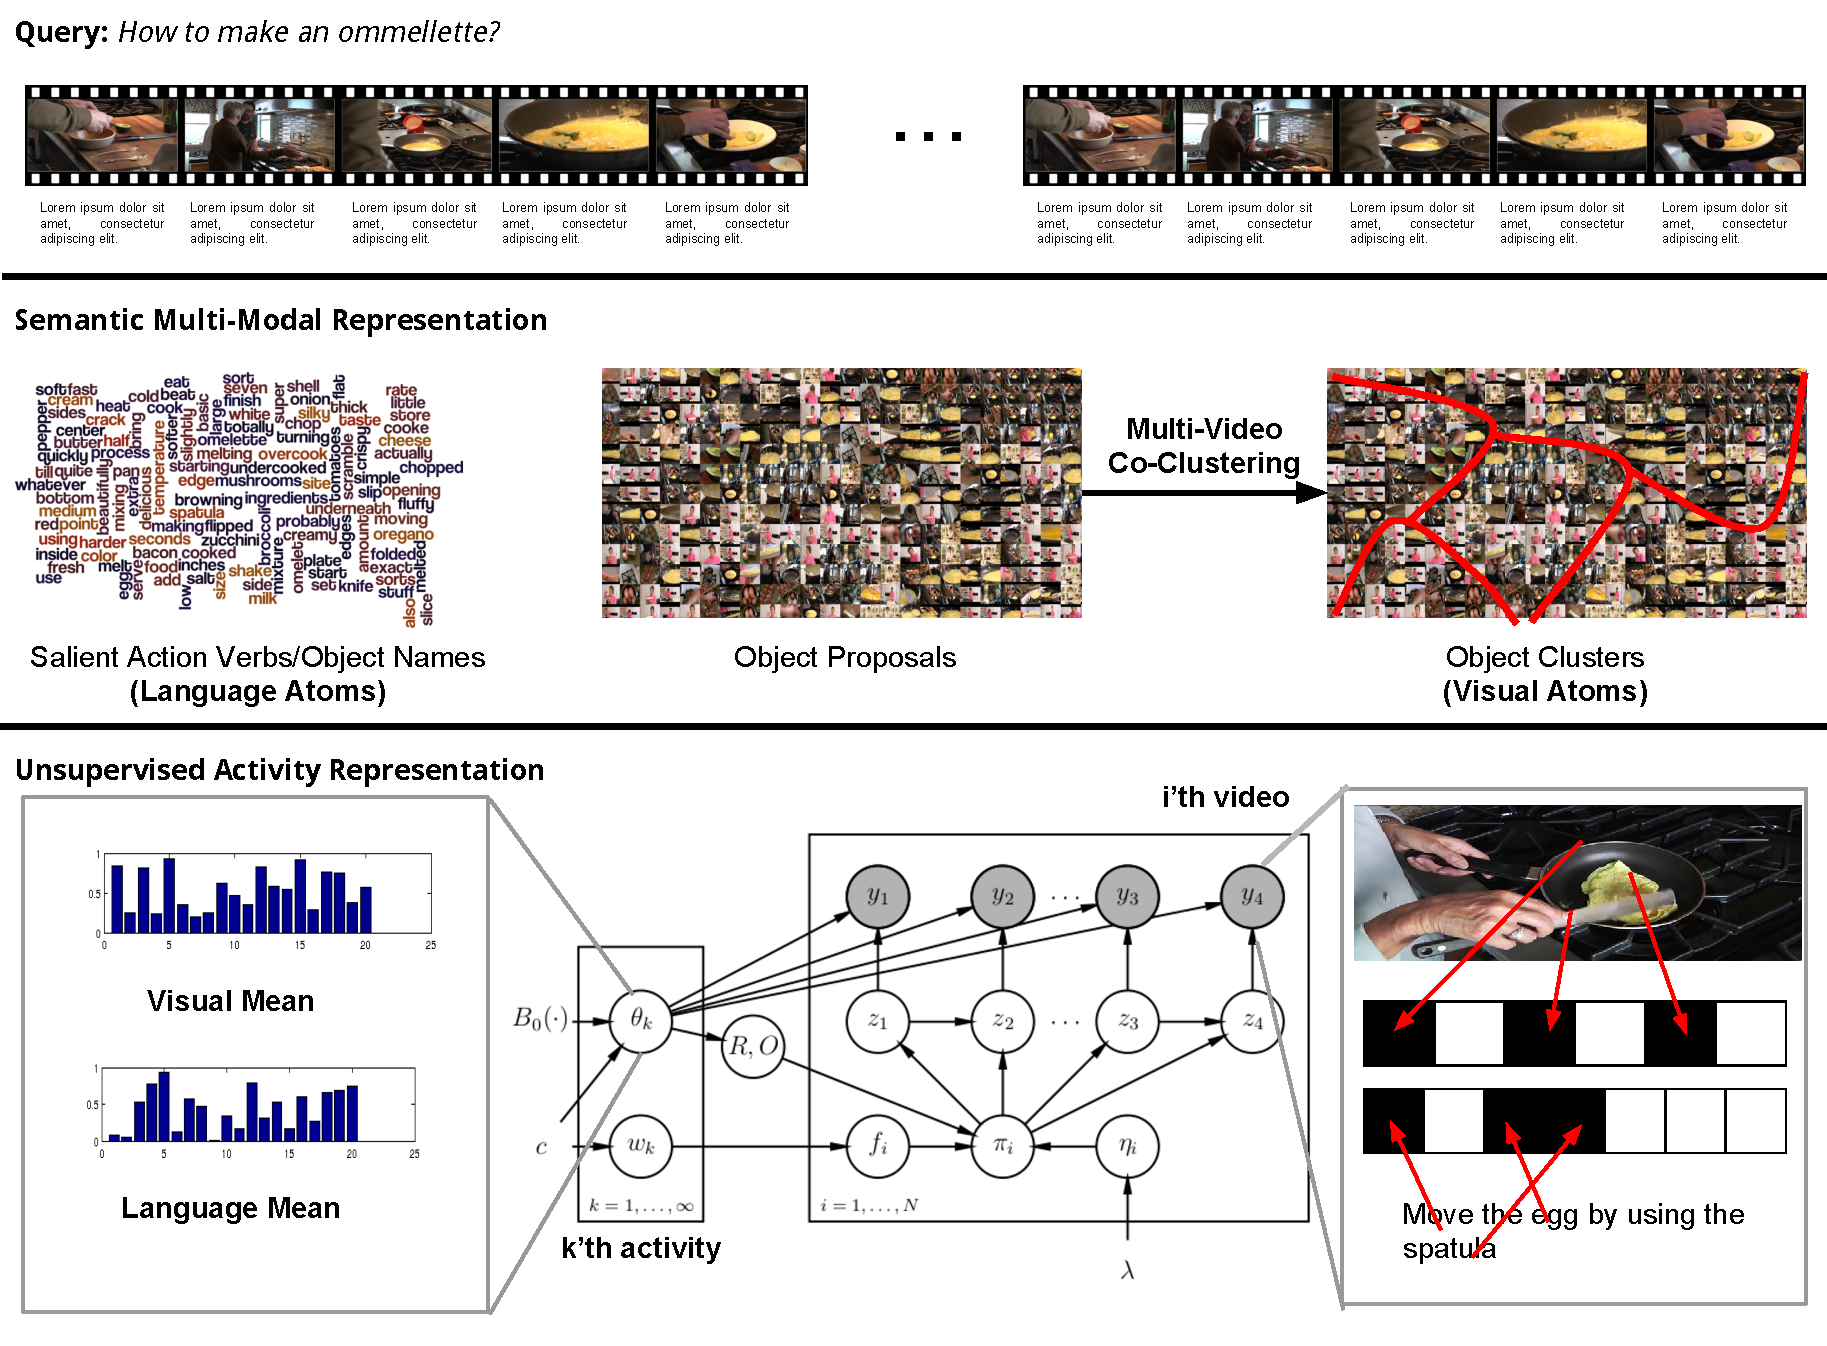
\includegraphics[width=\textwidth]{algor}
  \label{fig:overview}
  \caption{Components of our recipe understanding method. \textbf{Query:} We query the YouTube for top 100 \emph{How To} videos and filter the outliers; \textbf{Framewise Representation:} We automatically extract object clusters and salient word in order to find multi-modal representation of each frame. \textbf{Unsupervised Activity Detection:} We jointly cluster videos in order to learn activities/steps related to the recipe.}
\end{figure*}

In this section, we explain the high-level compenents of the method we develop to jointly represent multi-modal instructions. As shown in the Figure \ref{fig:overview}, our proposed method consists of three major components; online query and filtering, frame-wise multi-modal representation and joint clustering to extract activities. \textbf{(1) Query subsystem:} Our system starts with querying the YouTube with an \emph{How to} question for top 100 videos. The text descriptions of the returned videos are represented as bag-of-words and clustered to eliminate outliers. \textbf{(2) Framewise Representation:} In order to represent the frames of the returned videos, we process both the visual and language content of the videos. We extract the object proposals and jointly cluster them in order to detect the salient objects of the recipe. For the language descriptions, we use the top salient words of the courpus generated by concatenation of the all subtitles. We represent each frame in terms of the resulting salient objects and words. \textbf{(3) Unsupervised Activity Detection:} After describing each frame by using the salient objects and words, we apply a non-parametric Bayesian method in order to find the temporally consistent video clip clusters occuring over multiple videos. Our empirical results suggest that the resulting clusters mostly correspond to the activities. We now explain the details of the each sub-system in the following sections.
